\documentclass[11pt,a4paper]{article}
\usepackage[utf8]{inputenc}
\usepackage[vietnamese]{babel}
\usepackage{amsmath,amssymb}
\usepackage[version=4]{mhchem}
\usepackage{geometry}
\geometry{top=0.55cm,bottom=0.55cm,left=1.20cm,right=1.20cm,headheight=26pt,headsep=2pt,footskip=13pt}
\usepackage{graphicx}
\usepackage{xcolor}
\usepackage{tabularx}
\usepackage{array}
\usepackage{tikz}
\usepackage{multicol}
\usepackage{fancyhdr}
\usepackage{enumitem}

\definecolor{hfRed}{HTML}{D32F2F}
\definecolor{hfGreen}{HTML}{8BC390}
\definecolor{mainGreen}{HTML}{2E7D32}

\usepackage{ex_test}

\pagestyle{fancy}
\fancyhf{}
\renewcommand{\headrulewidth}{0.75pt}
\renewcommand{\headrule}{\hbox to\headwidth{\color{hfGreen}\leaders\hrule height \headrulewidth\hfill}}
\renewcommand{\footrulewidth}{0.75pt}
\renewcommand{\footrule}{\hbox to\headwidth{\color{hfGreen}\leaders\hrule height \footrulewidth\hfill}}

\fancyhead[L]{\small\itshape\color{hfRed}Tài liệu lưu hành nội bộ}
\fancyhead[R]{\small\color{hfRed}Thầy \textbf{TRẦN VĂN THẠNH} - 0777.470.803}

\fancyfoot[L]{\footnotesize\itshape\color{hfRed}CS1: 6/15 Nguyễn Hoàng, P. Kim Long, TP Huế \quad|\quad CS2: 24 Đặng Thái Thân, TP Huế}
\fancyfoot[R]{\small\textbf{\color{hfRed}Trang \thepage}}

\setlength{\parindent}{0pt}
\setlength{\parskip}{0.8pt}

\begin{document}

\begin{minipage}[t]{0.45\textwidth}
\textbf{SỞ GD\&ĐT THỪA THIÊN HUẾ}\\
\textbf{TRƯỜNG THPT HAI BÀ TRƯNG}\\
\textit{ĐỀ CHÍNH THỨC}\\
\textit{(Đề thi có 04 trang)}
\end{minipage}
\hfill
\begin{minipage}[t]{0.52\textwidth}
\raggedleft
\textbf{\color{hfRed}ĐỀ KIỂM TRA CHƯƠNG 8 -- NĂM HỌC 2026 - 2027}\\
\textbf{MÔN: HOÁ HỌC -- KHỐI 12}\\
\textit{Thời gian làm bài: 50 phút (không kể thời gian phát đề)}\\
\textbf{MÃ ĐỀ THI: 124}
\end{minipage}

\vspace{2pt}
\noindent
\textit{Họ, tên thí sinh:} \dotfill \textit{Lớp:} \dotfill \textit{SBD:} \dotfill

\vspace{1pt}
\noindent
\textit{\footnotesize (Cho biết nguyên tử khối: H = 1; C = 12; N = 14; O = 16; Na = 23; Mg = 24; Al = 27; S = 32; Cl = 35,5; K = 39; Ca = 40; Ti = 48; Cr = 52; Mn = 55; Fe = 56; Ni = 58,7; Cu = 64; Zn = 65; Ag = 108; Ba = 137; Pt = 195).}

\vspace{2pt}
\begin{center}
\textbf{\color{hfRed}\large (BẢN GIÁO VIÊN -- CÓ ĐÁP ÁN VÀ HƯỚNG DẪN GIẢI CHI TIẾT)}
\end{center}

\vspace{2pt}
\noindent
\textbf{PHẦN I (4,5 điểm -- 18 câu): Câu trắc nghiệm nhiều phương án lựa chọn.}\\
\textit{Thí sinh trả lời từ câu 1 đến câu 18. Mỗi câu hỏi thí sinh chỉ chọn một phương án.}

\Opensolutionfile{ans}[ans-de24-gv]

\begin{ex}
[KNTT - SBT] Nguyên tử Cr có cấu hình electron ở trạng thái cơ bản là $\text{[Ar]}3d^5 4s^1$. Trong phản ứng hoá học, khi nguyên tử Cr nhường đi 3 electron để tạo thành ion $\ce{Cr^3+}$, số electron còn lại trên phân lớp 3d là
\choice
{5.}
{4.}
{\True 3.}
{2.}
\loigiai{
Cấu hình electron của Cr: $\text{[Ar]}3d^5 4s^1$. Khi nhường 3 electron: nhường 1 electron ở phân lớp 4s và 2 electron ở phân lớp 3d, tạo cation $\ce{Cr^3+}$ có cấu hình $\text{[Ar]}3d^3$. Do đó số electron còn lại trên phân lớp 3d là 3.\\
\textbf{Chọn C.}}
\end{ex}

\begin{ex}
[KNTT - SBT] Dung dịch nào sau đây có màu vàng chanh?
\choice
{\ce{CuSO4}.}
{\True \ce{FeCl3}.}
{\ce{KMnO4}.}
{\ce{FeSO4}.}
\loigiai{
Dung dịch $\ce{FeCl3}$ có màu vàng chanh/vàng nâu đặc trưng (do sự thuỷ phân và tạo phức aqua của ion $\ce{Fe^3+}$). Dung dịch $\ce{CuSO4}$ màu xanh lam; $\ce{KMnO4}$ màu tím; $\ce{FeSO4}$ màu xanh lục nhạt.\\
\textbf{Chọn B.}}
\end{ex}

\begin{ex}
[KNTT - SBT] Dãy kim loại nào sau đây sắp xếp theo thứ tự tăng dần nhiệt độ nóng chảy?
\choice
{Na, Fe, Mg.}
{\True Na, Mg, Fe.}
{Fe, Mg, Na.}
{Mg, Fe, Na.}
\loigiai{
Nhiệt độ nóng chảy: Na ($97{,}8^\circ\text{C}$) < Mg ($650^\circ\text{C}$) < Fe ($1538^\circ\text{C}$). Dãy sắp xếp theo thứ tự tăng dần là Na, Mg, Fe.\\
\textbf{Chọn B.}}
\end{ex}

\begin{ex}
[CTST - SBT] Dung dịch muối chromium(III) sulfate có lẫn copper(II) sulfate, sử dụng dung dịch nào sau đây có thể loại bỏ nguyên tố copper ra khỏi muối chromium(III) sulfate?
\choice
{\True Dung dịch ammonia.}
{Dung dịch xút.}
{Dung dịch barium chloride.}
{Dung dịch soda.}
\loigiai{
Nhỏ dung dịch ammonia (\ce{NH3}) dư vào hỗn hợp: ion $\ce{Cu^2+}$ tạo phức chất tan $\ce{[Cu(NH3)4(H2O)2]^2+}$ có màu xanh thẫm, còn ion $\ce{Cr^3+}$ tạo kết tủa $\ce{Cr(OH)3}$ không tan trong ammonia dư. Lọc lấy kết tủa $\ce{Cr(OH)3}$, sau đó cho tác dụng với lượng vừa đủ dung dịch $\ce{H2SO4}$ loãng thu lại dung dịch $\ce{Cr2(SO4)3}$ tinh khiết.\\
\textbf{Chọn A.}}
\end{ex}

\begin{ex}
Phức chất là gì?
\choice
{Phức chất là những hợp chất có cấu tạo rất phức tạp.}
{Phức chất là những chất gồm nhiều phân tử chất đơn giản kết hợp lại.}
{Phức chất là những chất được tạo thành từ hai hay nhiều phân tử muối.}
{\True Phức chất là những chất khi phân li trong dung dịch tạo thành các ion phức tồn tại độc lập và có tính chất xác định.}
\loigiai{
Theo định nghĩa SGK Hoá học 12, phức chất là những chất khi phân li trong dung dịch tạo thành các ion phức (hoặc bản thân là phân tử phức trung hoà) tồn tại độc lập và có tính chất hoá học xác định.\\
\textbf{Chọn D.}}
\end{ex}

\begin{ex}
Cho phát biểu sau: “Phức chất đơn giản thường có một.(1). liên kết với các phối tử bao quanh. Liên kết giữa nguyên tử trung tâm và phối tử trong phức chất là liên kết.(2).”. Cụm từ cần điền vào (1) và (2) lần lượt là
\choice
{cation kim loại, ion.}
{nguyên tử kim loại, cho -- nhận.}
{\True nguyên tử trung tâm, cho -- nhận.}
{phối tử, ion.}
\loigiai{
Phức chất đơn giản có một nguyên tử trung tâm (1) liên kết với các phối tử bao quanh qua liên kết phối trí hay liên kết cho -- nhận (2).\\
\textbf{Chọn C.}}
\end{ex}

\begin{ex}
Phức chất nào sau đây chứa ion phức có số phối trí là 4?
\choice
{\True $\ce{[Zn(NH3)4]^2+}$.}
{$\ce{[Ag(NH3)2]+}$.}
{$\ce{[Co(NH3)6]^3+}$.}
{$\ce{[Ni(CN)4]^2-}$.}
\loigiai{
Trong ion phức $\ce{[Zn(NH3)4]^2+}$, nguyên tử trung tâm $\ce{Zn^2+}$ liên kết với 4 phối tử một càng \ce{NH3} nên có số phối trí là 4 (cấu trúc tứ diện). (Lưu ý: ion phức $\ce{[Ni(CN)4]^2-}$ cũng có số phối trí 4 dạng vuông phẳng).\\
\textbf{Chọn A.}}
\end{ex}

\begin{ex}
Trong phức chất $\ce{[Cr(H2O)6]Cl3}$, ion phức có dạng hình học gì?
\choice
{Hình vuông.}
{Lập phương.}
{\True Hình bát diện.}
{Hình tứ diện.}
\loigiai{
Cation phức $\ce{[Cr(H2O)6]^3+}$ có 6 phối tử nước liên kết với ion trung tâm $\ce{Cr^3+}$, có số phối trí 6 nên có cấu trúc hình học bát diện (octahedron).\\
\textbf{Chọn C.}}
\end{ex}

\begin{ex}
Chọn phát biểu sai:
\choice
{Phức chất có thể mang điện tích hoặc không mang điện tích.}
{\True Phức chất mà nguyên tử trung tâm tạo 4 liên kết với các phối tử luôn có dạng hình học là tứ diện.}
{Giống như phân tử ammonia, phân tử methylamine cũng có thể đóng vai trò là phối tử do có cặp electron chưa liên kết.}
{Phức có 4 phối tử và nguyên tử trung tâm có AO $d^8$ sẽ có dạng hình học vuông phẳng.}
\loigiai{
Phát biểu B sai vì phức chất có 4 phối tử có thể có cấu trúc tứ diện (như $\ce{[Zn(NH3)4]^2+}$) hoặc dạng vuông phẳng (như cisplatin $\ce{[Pt(NH3)2Cl2]}$, $\ce{[PtCl4]^2-}$, $\ce{[Ni(CN)4]^2-}$).\\
\textbf{Chọn B.}}
\end{ex}



\begin{ex}
Trong phương trình hoá học dạng tổng quát của phức chất aqua: $\ce{M^{n+}(aq) + m H2O(l) -> [M(OH2)_m]^{n+}(aq)}$. Giá trị $n$ là:
\choice
{số electron hoá trị của cation kim loại M.}
{\True giá trị điện tích của cation kim loại M.}
{số electron độc thân của cation kim loại M.}
{hoá trị của cation kim loại M.}
\loigiai{
Trong kí hiệu cation $\ce{M^{n+}}$, $n$ là độ lớn giá trị điện tích của cation kim loại M.\\
\textbf{Chọn B.}}
\end{ex}

\begin{ex}
Phản ứng tạo phức chất thường có một số dấu hiệu dễ quan sát như
\choice
{sự hoà tan, sự ngưng tụ.}
{sự biến đổi màu sắc, sự thay đổi nhiệt độ nóng chảy.}
{\True sự biến đổi màu sắc, sự hoà tan, sự kết tủa.}
{sự hoà tan, sự thay đổi nhiệt độ sôi.}
\loigiai{
Dấu hiệu đặc trưng nhận biết phản ứng tạo phức chất trong dung dịch là sự biến đổi màu sắc dung dịch, sự hoà tan kết tủa hoặc xuất hiện kết tủa màu đặc trưng.\\
\textbf{Chọn C.}}
\end{ex}

\begin{ex}
Cho dung dịch ammonia dư vào dung dịch chứa phức chất $\ce{[Ni(OH2)6]^2+}$ và anion $\ce{Cl-}$, có phản ứng: $\ce{[Ni(OH2)6]^2+(aq) + 6NH3(aq) -> [Ni(NH3)6]^2+(aq) + 6H2O(l)}$ (*). Phát biểu nào sau đây không đúng?
\choice
{\True Trong điều kiện của phản ứng (*), phức chất $\ce{[Ni(NH3)6]^2+}$ kém bền hơn phức chất $\ce{[Ni(OH2)6]^2+}$.}
{Phản ứng (*) là phản ứng thế phối tử.}
{Dung dịch sau phản ứng có $\text{pH} > 7$.}
{Trong phản ứng không có sự thay đổi số oxi hoá của các nguyên tố.}
\loigiai{
Phản ứng (*) diễn ra thuận lợi theo chiều thuận chứng tỏ phức chất amine $\ce{[Ni(NH3)6]^2+}$ bền hơn phức chất aqua $\ce{[Ni(OH2)6]^2+}$. Phát biểu A nói phức amine kém bền hơn là sai.\\
\textbf{Chọn A.}}
\end{ex}

\begin{ex}
Nhỏ vài giọt dung dịch \ce{NH3} vào dung dịch \ce{CuSO4} loãng thấy xuất hiện kết tủa màu xanh nhạt, chứng tỏ phức chất $\ce{[Cu(OH)2(H2O)4]}$ đã được tạo thành. Tiếp tục nhỏ vào ống nghiệm dung dịch \ce{NH3} đến dư thấy kết tủa tan, đồng thời dung dịch chuyển sang màu xanh lam, chứng tỏ phức chất $\ce{[Cu(NH3)4(H2O)2]^2+}$ đã được tạo thành. Dấu hiệu của phản ứng tạo phức trên dựa vào:
\choice
{sự biến đổi màu sắc.}
{\True sự biến đổi màu sắc và sự hoà tan.}
{sự hoà tan.}
{sự kết tủa.}
\loigiai{
Quá trình cho \ce{NH3} đến dư có hiện tượng kết tủa tan dần và dung dịch đổi màu từ xanh nhạt sang xanh lam thẫm, do đó dựa vào sự biến đổi màu sắc và sự hoà tan kết tủa.\\
\textbf{Chọn B.}}
\end{ex}

\begin{ex}
Phản ứng chuẩn độ $\ce{Fe^2+}$ trong dung dịch acid bằng dung dịch \ce{KMnO4} được biểu diễn bởi phương trình ion rút gọn sau: $\ce{MnO4-(aq) + 5Fe^2+(aq) + 8H+(aq) -> Mn^2+(aq) + 5Fe^3+(aq) + 4H2O(l)}$. Chất oxi hoá trong phản ứng trên là
\choice
{$\ce{Fe^2+(aq)}$.}
{$\ce{Mn^2+(aq)}$.}
{\True $\ce{MnO4-(aq)}$.}
{$\ce{H+(aq)}$.}
\loigiai{
Trong phản ứng, ion permanganate $\ce{MnO4-}$ có nguyên tử Mn(+7) nhận 5 electron giảm xuống Mn(+2) nên đóng vai trò là chất oxi hoá. $\ce{Fe^2+}$ nhường 1 electron là chất khử.\\
\textbf{Chọn C.}}
\end{ex}

\begin{ex}
Có thể loại bỏ sắt trong nước ngầm bằng cách đưa nước ngầm lên các bể lắng, lọc và sục không khí vào. Khi đó $\ce{Fe^2+}$ trong nước ngầm bị chuyển thành $\ce{Fe(OH)3}$ và lắng xuống. Chất oxi hoá $\ce{Fe^2+}$ thành $\ce{Fe(OH)3}$ là
\choice
{\True khí \ce{O2}.}
{khí \ce{N2}.}
{nước và khí \ce{O2}.}
{khí \ce{O2} và \ce{OH-}.}
\loigiai{
Khí oxygen (\ce{O2}) trong không khí sục vào đóng vai trò là chất oxi hoá: $4\ce{Fe^2+} + \ce{O2} + 10\ce{H2O} \rightarrow 4\ce{Fe(OH)3}\downarrow + 8\ce{H+}$. Trong đó số oxi hoá của oxygen giảm từ 0 xuống -2.\\
\textbf{Chọn A.}}
\end{ex}

\begin{ex}
\begin{minipage}[t]{0.74\textwidth}
Phức chất $\ce{[Fe(OH2)6]^3+}$ có cấu tạo như hình bên. Số liên kết cho -- nhận mà nguyên tử trung tâm iron tạo được với các phối tử $\ce{OH2}$ là
\choice
{5.}
{4.}
{3.}
{\True 6.}
\end{minipage}\hfill
\begin{minipage}[t]{0.24\textwidth}
\centering\vspace{0pt}
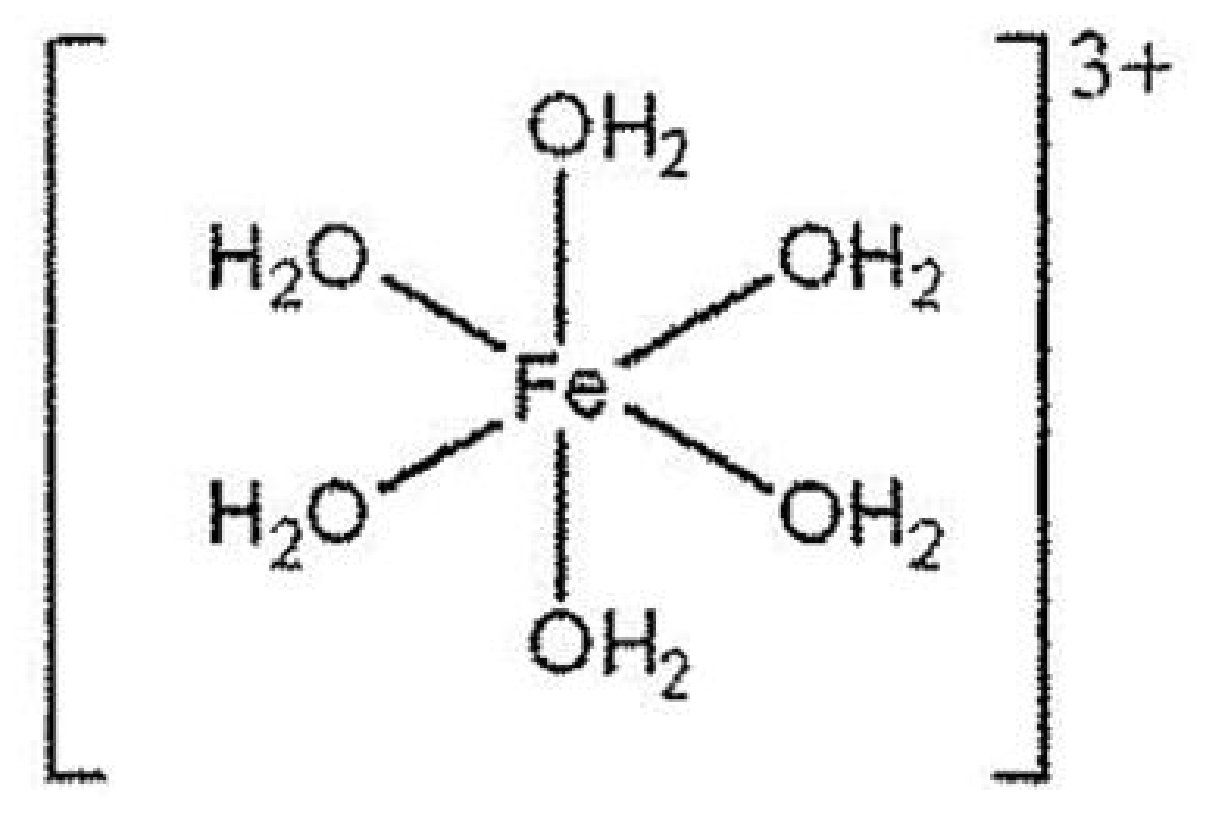
\includegraphics[width=\linewidth]{images_crop_de24/p1_cau16_fe_oh2_6.png}
\end{minipage}
\loigiai{
Cation trung tâm $\ce{Fe^3+}$ liên kết với 6 phối tử nước $\ce{OH2}$ qua 6 liên kết cho -- nhận (phối trí) tạo nên cấu trúc hình học bát diện.\\
\textbf{Chọn D.}
}
\end{ex}

\begin{ex}
Trong các số oxi hoá của các kim loại chuyển tiếp dãy thứ nhất, trạng thái thường gặp nhất là +2. Điều này được giải thích là do đa số các kim loại chuyển tiếp dãy thứ nhất có độ âm điện không cao và
\choice
{dễ nhường đi 2 electron ở phân lớp 3d.}
{dễ nhường đi 1 electron ở phân lớp 3d và 1 electron ở phân lớp 4s.}
{có khả năng nhận thêm 2 electron vào phân lớp 3d.}
{\True có 2 electron lớp ngoài cùng.}
\loigiai{
Các nguyên tử kim loại chuyển tiếp dãy thứ nhất có cấu hình electron hoá trị là $3d^n 4s^2$, lớp electron ngoài cùng có 2 electron ở phân lớp 4s dễ nhường đi để tạo cation mang số oxi hoá +2.\\
\textbf{Chọn D.}}
\end{ex}

\begin{ex}
Một học sinh tiến hành chuẩn độ dung dịch $\ce{Fe^2+}$ bằng dung dịch \ce{KMnO4} theo 2 cách:\\
-- \textit{Cách 1:} Nhỏ từ từ dung dịch \ce{KMnO4} vào dung dịch $\ce{Fe^2+}$ trong acid đến khi xuất hiện màu hồng nhạt bền khoảng 30 giây.\\
-- \textit{Cách 2:} Nhỏ từ từ dung dịch $\ce{Fe^2+}$ trong acid vào dung dịch \ce{KMnO4} đến khi màu hồng biến mất.\\
Cách tiến hành chuẩn độ nào là phù hợp?
\choice
{\True Cách 1.}
{Cách 2.}
{Cả hai cách.}
{Không có cách nào.}
\loigiai{
Trong chuẩn độ permanganate, dung dịch chất chuẩn \ce{KMnO4} nạp vào buret và nhỏ từng giọt vào bình tam giác chứa $\ce{Fe^2+}$. Điểm tương đương được nhận biết nhạy và chính xác khi 1 giọt \ce{KMnO4} dư làm dung dịch đổi từ không màu sang màu hồng nhạt bền trong khoảng 30 giây (Cách 1). Ngược lại, Cách 2 nhỏ $\ce{Fe^2+}$ vào \ce{KMnO4} quan sát thời điểm mất màu hồng rất khó chính xác.\\
\textbf{Chọn A.}}
\end{ex}



\noindent
\textbf{PHẦN II (4,0 điểm -- 4 câu): Câu trắc nghiệm đúng sai.}\\
\textit{Thí sinh trả lời từ câu 1 đến câu 4. Trong mỗi ý a), b), c), d) ở mỗi câu, thí sinh chọn đúng hoặc sai.}

\setcounter{ex}{0}

\begin{ex}
\begin{minipage}[t]{0.70\textwidth}
Titanium (Ti) được sử dụng để chế tạo động cơ hoặc khung máy bay, còn titanium dioxide ($\ce{TiO2}$) được sử dụng trong sản xuất kem chống nắng. Quặng ilmenite ($\ce{FeTiO3}$) có giá trị quan trọng về mặt kinh tế để sản xuất kim loại titanium. $\ce{TiO2}$ sản xuất từ $\ce{FeTiO3}$ (phản ứng A), sau đó được chuyển hoá thành Ti theo quy trình Kroll (phản ứng B, C, D) như hình bên.\\
Xét tính đúng/sai của các phát biểu sau:
\choiceTF
{\True Phương trình hoá học của phản ứng A là: $\ce{FeTiO3 + C -> Fe + TiO2 + CO}$.}
{Phương trình hoá học của phản ứng B là: $\ce{TiO2 + 2Cl2 -> TiCl4 + O2}$.}
{\True Phương trình hoá học của phản ứng C là: $\ce{TiCl4 + 2Mg -> 2MgCl2 + Ti}$.}
{\True Phương trình tổng cộng của 4 phản ứng là: $\ce{FeTiO3 + 3C -> Fe + Ti + 3CO}$.}
\end{minipage}\hfill
\begin{minipage}[t]{0.28\textwidth}
\centering\vspace{0pt}
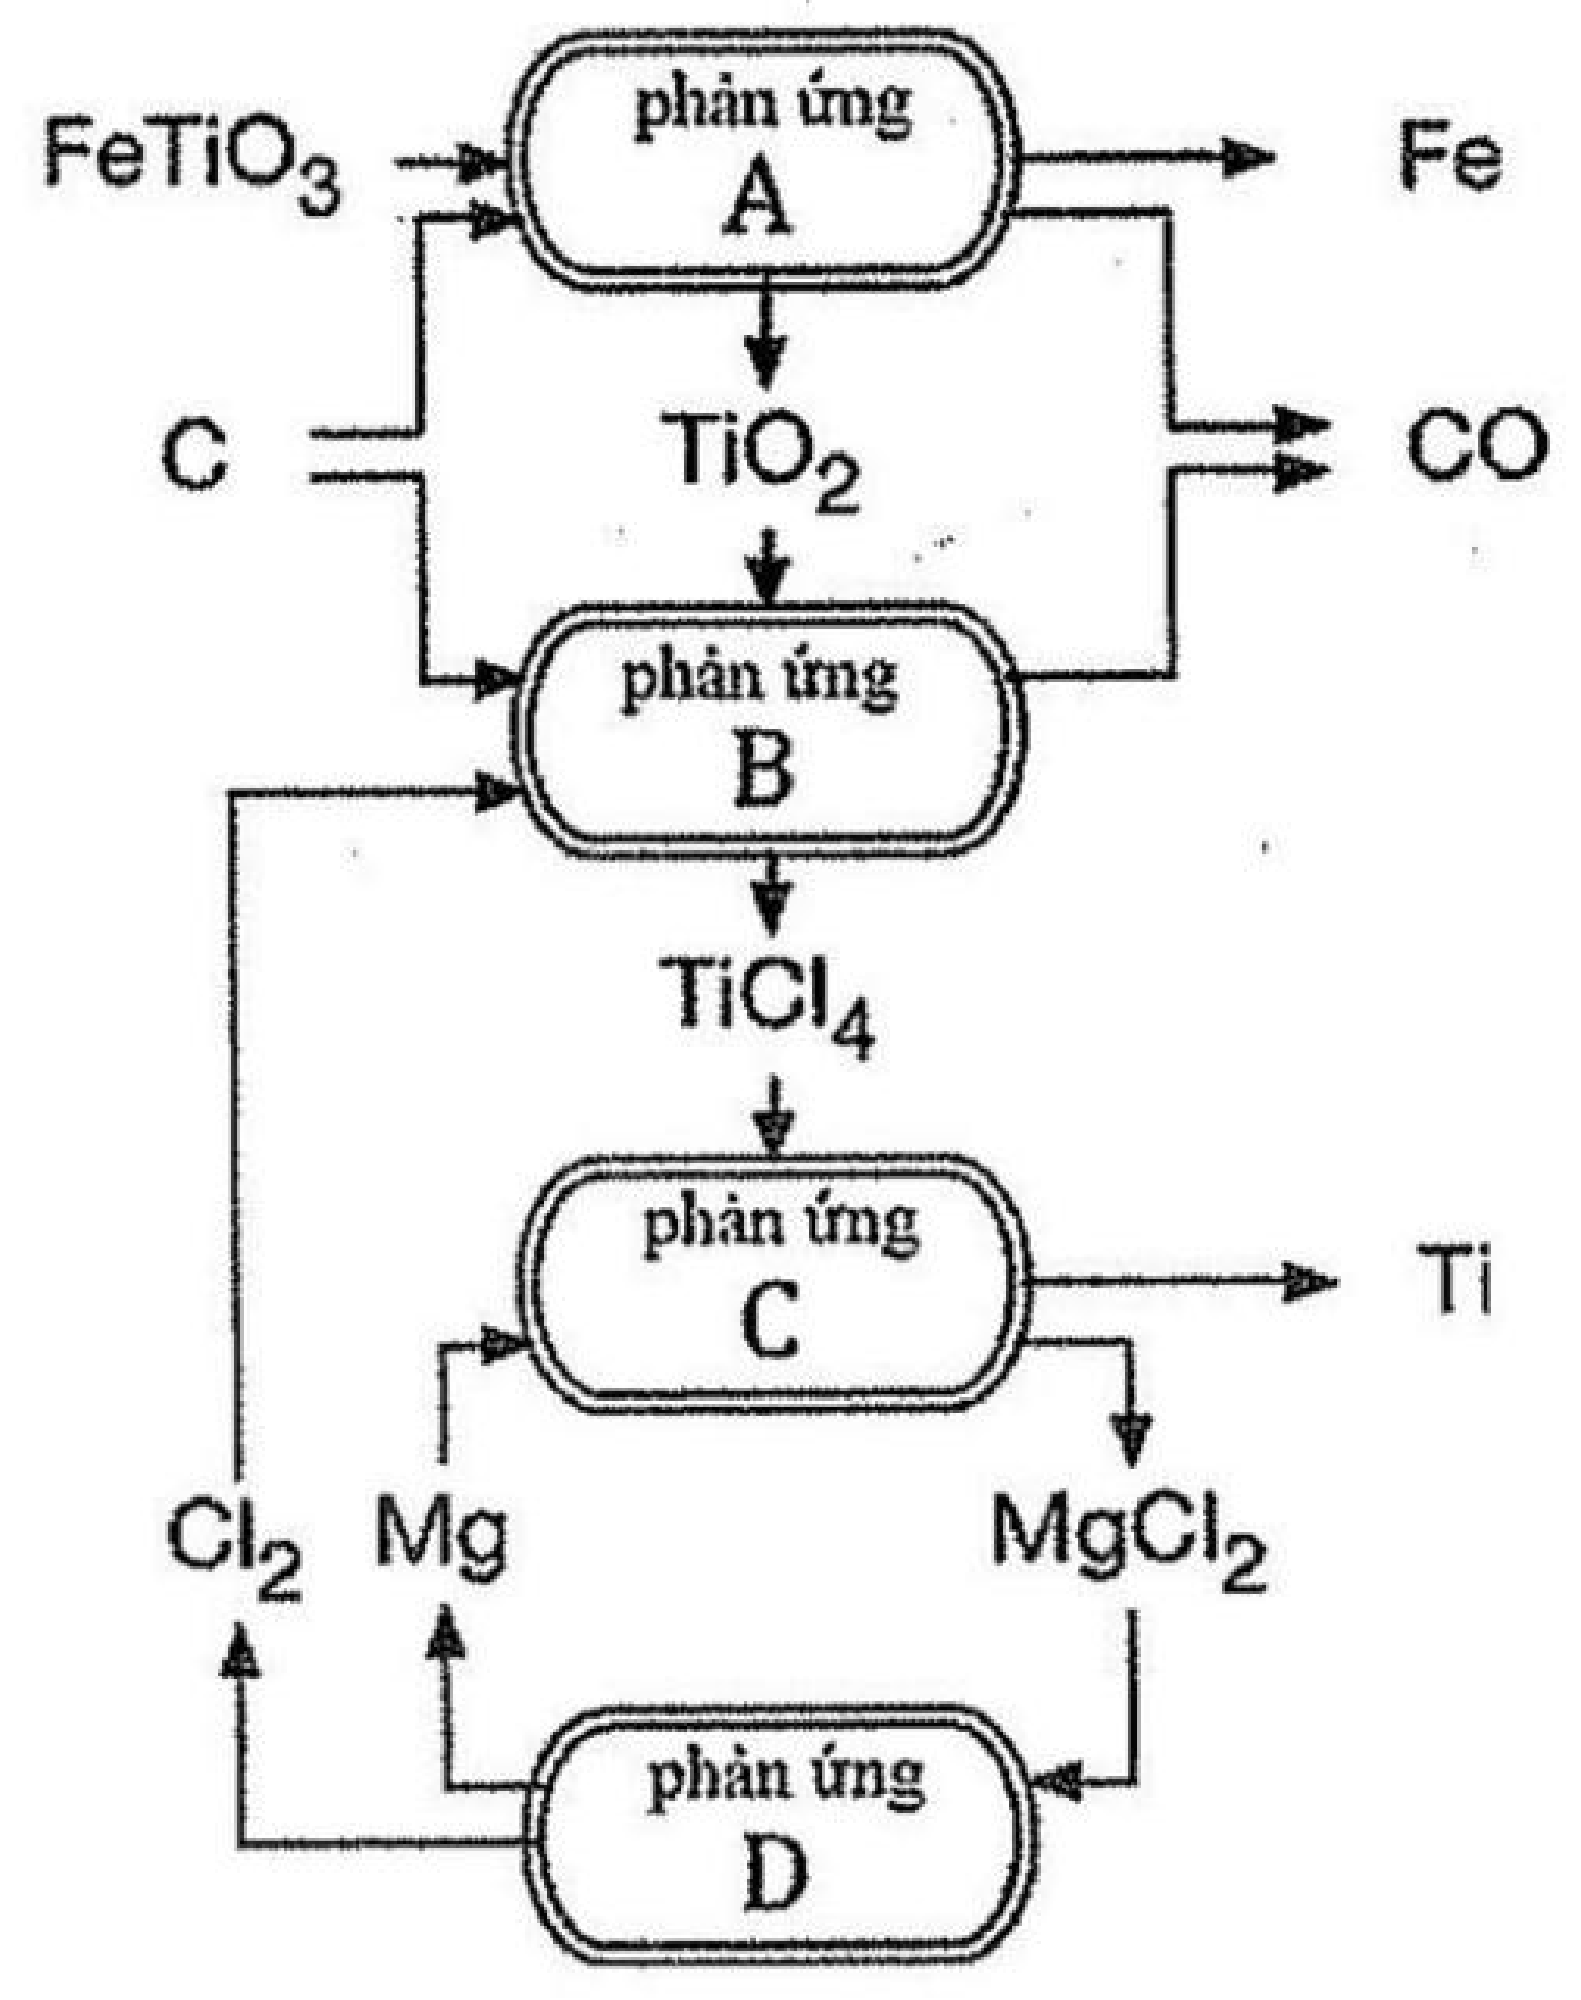
\includegraphics[width=\linewidth]{images_crop_de24/p2_cau1_quy_trinh_kroll.png}
\end{minipage}
\loigiai{
a) \textbf{Đúng.} Quá trình hoàn nguyên nhiệt cacbon có chọn lọc quặng ilmenite tạo kim loại Fe và $\ce{TiO2}$.\\
b) \textbf{Sai.} Phản ứng chlorine hoá $\ce{TiO2}$ cần có mặt carbon ở nhiệt độ cao: $\ce{TiO2 + 2C + 2Cl2 -> TiCl4 + 2CO}$, không sinh ra $\ce{O2}$.\\
c) \textbf{Đúng.} Khử $\ce{TiCl4}$ bằng kim loại Mg nóng chảy trong khí trơ argon ở khoảng 800 -- $850^\circ\text{C}$.\\
d) \textbf{Đúng.} Phản ứng D là điện phân nóng chảy tái chế $\ce{MgCl2 -> Mg + Cl2}$; cộng cả 4 phản ứng thu được: $\ce{FeTiO3 + 3C -> Fe + Ti + 3CO}$.
}
\end{ex}

\begin{ex}
Phức chất \textit{cis}-$\ce{[Pt(NH3)2Cl2]}$ là một hợp chất vô cơ có khả năng ức chế các tế bào ung thư như ung thư tinh hoàn, buồng trứng, bàng quang và các khối u ở đầu và cổ. Mỗi phát biểu sau là đúng hay sai?
\choiceTF
{Ion trung tâm là Pt.}
{Phối tử là \ce{NH3}.}
{\True Ion trung tâm là $\ce{Pt^2+}$, phối tử là \ce{NH3} và \ce{Cl-}.}
{\True Phức có dạng hình học là vuông phẳng.}
\loigiai{
a) \textbf{Sai.} Cation trung tâm là ion $\ce{Pt^2+}$ (nguyên tử Pt ở trạng thái oxi hoá +2).\\
b) \textbf{Sai.} Phối tử gồm cả 2 phân tử \ce{NH3} và 2 ion \ce{Cl-}; phát biểu chỉ nêu \ce{NH3} là chưa đầy đủ.\\
c) \textbf{Đúng.} Cation trung tâm là $\ce{Pt^2+}$, các phối tử liên kết là \ce{NH3} và \ce{Cl-}.\\
d) \textbf{Đúng.} Phức chất cisplatin có dạng hình học vuông phẳng (square planar).
}
\end{ex}

\begin{ex}
[KNTT - SBT] Trong dung dịch, ion $\ce{Fe^3+}$ tồn tại dưới dạng phức chất aqua có sáu phối tử nước. Xét tính đúng/sai của các phát biểu sau:
\choiceTF
{\True Phức chất aqua có công thức hoá học là $\ce{[Fe(H2O)6]^3+}$.}
{Phức chất aqua có dạng hình học vuông phẳng.}
{\True 6 phối tử nước đã cho cặp electron chưa liên kết vào ion $\ce{Fe^3+}$.}
{Nguyên tử trung tâm trong phức chất aqua là $\ce{Fe^2+}$.}
\loigiai{
a) \textbf{Đúng.} Phức chất aqua của sắt(III) có công thức là $\ce{[Fe(H2O)6]^3+}$.\\
b) \textbf{Sai.} Phức có 6 phối tử nước nên có dạng hình học bát diện (octahedral).\\
c) \textbf{Đúng.} Mỗi phân tử nước dùng 1 cặp electron chưa liên kết của nguyên tử O để tạo liên kết phối trí với cation $\ce{Fe^3+}$.\\
d) \textbf{Sai.} Ion trung tâm là $\ce{Fe^3+}$, không phải $\ce{Fe^2+}$.
}
\end{ex}

\begin{ex}
Cho hai phức chất A và B có công thức cấu tạo lần lượt sau:
\par\vspace{1pt}\centerline{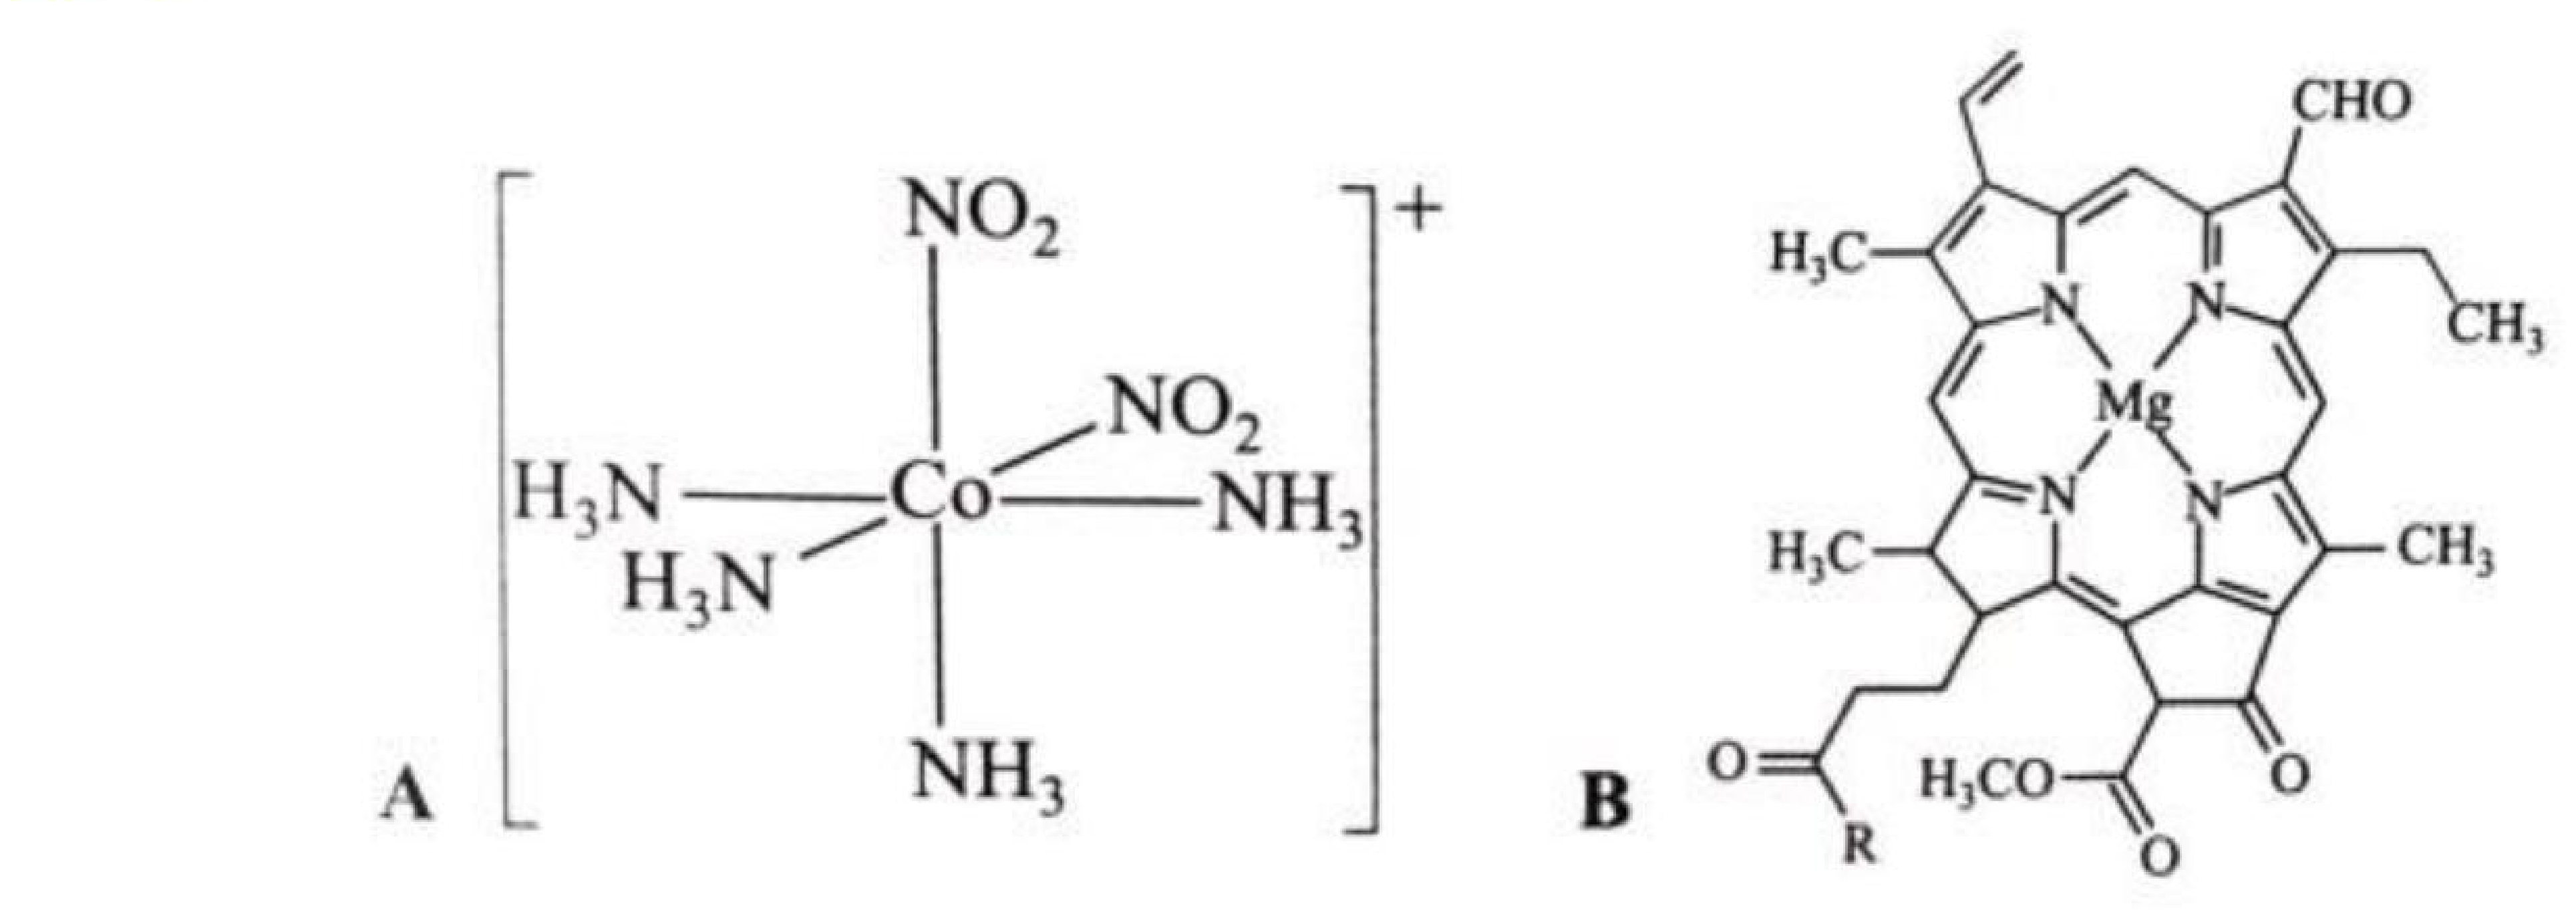
\includegraphics[height=2.3cm]{images_crop_de24/p2_cau4_phuc_A_B.png}}\vspace{1pt}
Mỗi phát biểu sau đây đúng hay sai?
\choiceTF
{Nguyên tử trung tâm của hai phức chất đều là nguyên tố kim loại chuyển tiếp.}
{Trong phức chất B có 4 phối tử.}
{\True Hai phức chất A và B có dạng hình học khác nhau.}
{Trong A và trong B đều có hai loại phối tử.}
\loigiai{
a) \textbf{Sai.} Phức A có nguyên tử trung tâm là Co (kim loại chuyển tiếp), còn phức B (chlorophyll) có nguyên tử trung tâm là Mg (kim loại kiềm thổ thuộc nhóm IIA -- nhóm chính, không phải kim loại chuyển tiếp).\\
b) \textbf{Sai.} Trong chlorophyll B chỉ có 1 phối tử vòng 4 càng porphyrin liên kết qua 4 nguyên tử N, không phải 4 phối tử độc lập.\\
c) \textbf{Đúng.} Phức A có dạng hình học bát diện, còn phức B có dạng phẳng vòng càng (square planar quanh nguyên tử Mg).\\
d) \textbf{Sai.} Phức A có 2 loại phối tử (\ce{NH3} và \ce{NO2-}), nhưng phức B chỉ có 1 loại phối tử là dẫn xuất chlorin/porphyrin.
}
\end{ex}



\noindent
\textbf{PHẦN III (1,5 điểm -- 6 câu): Câu trắc nghiệm yêu cầu trả lời ngắn.}\\
\textit{Thí sinh trả lời từ câu 1 đến câu 6.}

\setcounter{ex}{0}

\begin{ex}
\begin{minipage}[t]{0.70\textwidth}
Phức chất $\ce{[Co(NH3)4Cl2]+}$ có cấu trúc như hình bên:\\
Có bao nhiêu liên kết sigma ($\sigma$) có trong phức chất đó?
\end{minipage}\hfill
\begin{minipage}[t]{0.28\textwidth}
\centering\vspace{0pt}
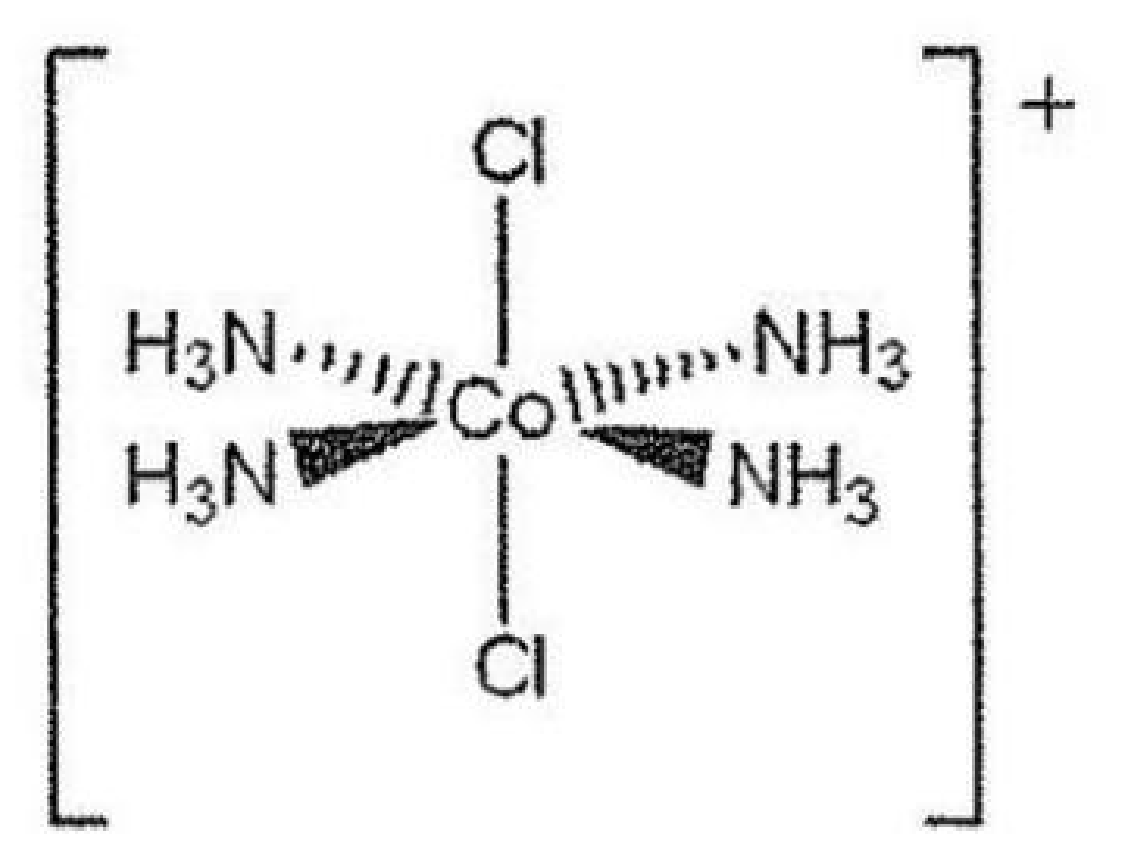
\includegraphics[height=1.8cm]{images_crop_de24/p3_cau1_co_nh3_4_cl2.png}
\end{minipage}
\loigiai{
• Trong 4 phối tử \ce{NH3}: mỗi phân tử \ce{NH3} có 3 liên kết đơn $\text{N-H}$ (liên kết $\sigma$), tổng cộng $4 \times 3 = 12$ liên kết $\sigma$ $\text{N-H}$.\\
• Cation trung tâm Co liên kết với 4 nguyên tử N qua 4 liên kết phối trí $\text{Co-N}$ (đều là liên kết $\sigma$).\\
• Cation trung tâm Co liên kết với 2 ion \ce{Cl-} qua 2 liên kết $\text{Co-Cl}$ (đều là liên kết $\sigma$).\\
• Tổng số liên kết $\sigma$ trong phức chất $= 12 + 4 + 2 = 18$ liên kết $\sigma$.\\
\textbf{Đáp số: 18.}
}
\end{ex}

\begin{ex}
[KNTT - SBT] Phức chất $\ce{[MA_x B2]}$ có dạng hình học bát diện. Ở đó M là nguyên tử trung tâm, $x$ là số phối tử của A. Giá trị của $x$ là bao nhiêu?
\loigiai{
Phức chất có dạng hình học bát diện nên có số phối trí là 6. Với các phối tử một càng A và B, tổng số phối tử là $x + 2 = 6 \Rightarrow x = 4$.\\
\textbf{Đáp số: 4.}}
\end{ex}


\begin{ex}
[KNTT - SBT] Phức chất $\ce{[Co(NH3)Cl_x]^y-}$ có dạng hình học bát diện, nguyên tử trung tâm là $\ce{Co^3+}$. Tổng giá trị của $x$ và $y$ là bao nhiêu?
\loigiai{
• Phức bát diện có tổng số phối tử một càng là $1 + x = 6 \Rightarrow x = 5$.\\
• Điện tích ion phức: $\ce{Co^3+}$ (+3), \ce{NH3} (0), 5 phối tử \ce{Cl-} (-5) $\Rightarrow$ điện tích ion phức là $(+3) + 0 + 5\times(-1) = -2 \Rightarrow y = 2$.\\
• Tổng giá trị của $x$ và $y = 5 + 2 = 7$.\\
\textbf{Đáp số: 7.}}
\end{ex}


\begin{ex}
[KNTT - SBT] Cho dung dịch \ce{NH3} đặc vào dung dịch phức chất $\ce{[PtCl4]^2-}$ thu được phức chất có điện tích +1 là do một số phối tử \ce{Cl-} trong phức $\ce{[PtCl4]^2-}$ bị thay thế bởi phối tử \ce{NH3}. Số lượng phối tử \ce{Cl-} đã bị thay thế là bao nhiêu?
\loigiai{
• Trong $\ce{[PtCl4]^2-}$, nguyên tử trung tâm Pt có số oxi hoá +2.\\
• Khi thay $k$ phối tử \ce{Cl-} bằng $k$ phân tử trung hoà \ce{NH3}, phức chất mới có dạng $\ce{[Pt(NH3)_k Cl_{4-k}]^{(k-2)+}}$.\\
• Điện tích phức chất mới bằng $+1 \Rightarrow k - 2 = +1 \Rightarrow k = 3$.\\
• Vậy số lượng phối tử \ce{Cl-} bị thay thế là 3 (tạo ra phức chất $\ce{[Pt(NH3)3Cl]+}$).\\
\textbf{Đáp số: 3.}}
\end{ex}


\begin{ex}
Sự gia tăng hàm lượng nitrate trong nước là một trong những nguyên nhân của hiện tượng phú dưỡng. Một trong những quy trình xác định hàm lượng nitrate trong nước được thực hiện như sau:\\
Thí nghiệm 1. Lấy 10,0 mL dung dịch muối Mohr [$\ce{(NH4)2SO4.FeSO4.6H2O}$], thêm $\ce{H2SO4}$ 1M vào và chuẩn độ bằng dung dịch \ce{KMnO4}.\\
Thí nghiệm 2. Lấy 10,0 mL dung dịch muối Mohr cho vào 100 mL nước chứa ion nitrate, sau đó thêm $\ce{NaOH(s)}$ vào để đạt khoảng 28\%, khi đó muối Mohr khử nitrate thành ammonia theo các phản ứng:\\
$\ce{NO3-(aq) + 2Fe(OH)2 + H2O -> NO2-(aq) + 2Fe(OH)3}$ (1)\\
$\ce{NO2-(aq) + 6Fe(OH)2 + 5H2O -> NH3 + 6Fe(OH)3 + OH-}$ (2)\\
Sau khi các phản ứng (1) và (2) hoàn toàn, lọc bỏ kết tủa, acid hoá dung dịch bằng dung dịch $\ce{H2SO4}$ 1M và chuẩn độ lượng $\ce{Fe^2+}$ dư bằng dung dịch \ce{KMnO4} (các chất và ion khác trong dung dịch không phản ứng với \ce{KMnO4}).\\
Hãy cho biết mỗi mmol \ce{KMnO4} chênh lệch giữa thí nghiệm 1 với thí nghiệm 2 sẽ tương ứng với bao nhiêu mg $\ce{NO3-}$ trong nước? \textit{(Làm tròn kết quả đến hàng phần mười)}.
\loigiai{
• Ở TN1: $5\ce{Fe^2+} + \ce{MnO4-} + 8\ce{H+} \rightarrow 5\ce{Fe^3+} + \ce{Mn^2+} + 4\ce{H2O} \Rightarrow 1\text{ mmol } \ce{KMnO4}$ tương ứng $5\text{ mmol } \ce{Fe^2+}$.\\
• Ở TN2: Cộng 2 phương trình khử $\ce{NO3-}$:\\
$\ce{NO3- + 8Fe(OH)2 + 6H2O -> NH3 + 8Fe(OH)3 + OH-} \Rightarrow 1\text{ mmol } \ce{NO3-}$ phản ứng với $8\text{ mmol } \ce{Fe^2+}$.\\
• Lượng \ce{KMnO4} chênh lệch: $\Delta n_{\ce{KMnO4}} = \dfrac{n_{\ce{Fe^2+ (p/u)}}}{5} = \dfrac{8}{5} n_{\ce{NO3-}} = 1{,}6\, n_{\ce{NO3-}} \Rightarrow n_{\ce{NO3-}} = \dfrac{\Delta n_{\ce{KMnO4}}}{1{,}6} = 0{,}625\, \Delta n_{\ce{KMnO4}}$.\\
• Với mỗi 1 mmol \ce{KMnO4} chênh lệch: $m_{\ce{NO3-}} = 0{,}625 \times 62 = 38{,}75\text{ mg} \approx 38{,}8\text{ mg}$.\\
\textbf{Đáp số: 38,8.}}
\end{ex}


\begin{ex}
Chromium (Cr) có tính cứng cao. Nickel (Ni) có đặc tính cơ học là cứng, dễ dát mỏng, dễ uốn, dễ kéo sợi và đặc tính hoá học là trơ với không khí nên khi thêm vào inox để việc gia công dễ dàng hơn. Inox 18/10 có thành phần hoá học gồm 18\% chromium, 10\% nickel và tối đa 0,08\% carbon (C). Xác định khối lượng iron (tính theo kg) tối đa trong 1,00 tấn inox 18/10.
\loigiai{
• Trong 1,00 tấn (1000 kg) inox 18/10 có: 18\% Cr, 10\% Ni, tối đa 0,08\% C và phần còn lại là Fe.\\
• Để khối lượng iron (Fe) đạt tối đa thì hàm lượng carbon và các tạp chất khác phải ở mức tối thiểu bằng 0\%.\\
• Khi đó \% khối lượng iron tối đa là: $\%m_{\ce{Fe (max)}} = 100\% - 18\% - 10\% = 72\%$.\\
• Khối lượng iron tối đa thu được là: $m_{\ce{Fe (max)}} = 1000 \times 72\% = 720\text{ kg}$.\\
\textbf{Đáp số: 720.}}
\end{ex}


\Closesolutionfile{ans}

\newpage
\begin{center}
\textbf{\Large\color{hfRed}BẢNG TỔNG HỢP ĐÁP ÁN ĐỀ SỐ 24}
\end{center}

\vspace{0.2cm}
\noindent\textbf{\color{mainGreen}PHẦN I (Mỗi câu trả lời đúng được 0,25 điểm)}
\begin{center}
\renewcommand{\arraystretch}{1.2}
\begin{tabular}{|c|c|c|c|c|c|c|c|c|c|}
\hline
\textbf{Câu 1} & \textbf{Câu 2} & \textbf{Câu 3} & \textbf{Câu 4} & \textbf{Câu 5} & \textbf{Câu 6} & \textbf{Câu 7} & \textbf{Câu 8} & \textbf{Câu 9} \\
\hline
\textbf{\color{hfRed}C} & \textbf{\color{hfRed}B} & \textbf{\color{hfRed}B} & \textbf{\color{hfRed}A} & \textbf{\color{hfRed}D} & \textbf{\color{hfRed}C} & \textbf{\color{hfRed}A} & \textbf{\color{hfRed}C} & \textbf{\color{hfRed}B} \\
\hline
\textbf{Câu 10} & \textbf{Câu 11} & \textbf{Câu 12} & \textbf{Câu 13} & \textbf{Câu 14} & \textbf{Câu 15} & \textbf{Câu 16} & \textbf{Câu 17} & \textbf{Câu 18} \\
\hline
\textbf{\color{hfRed}B} & \textbf{\color{hfRed}C} & \textbf{\color{hfRed}A} & \textbf{\color{hfRed}B} & \textbf{\color{hfRed}C} & \textbf{\color{hfRed}A} & \textbf{\color{hfRed}D} & \textbf{\color{hfRed}D} & \textbf{\color{hfRed}A} \\
\hline
\end{tabular}
\end{center}

\vspace{0.2cm}
\noindent\textbf{\color{mainGreen}PHẦN II (Đúng 1 ý: 0,1 đ; đúng 2 ý: 0,25 đ; đúng 3 ý: 0,5 đ; đúng 4 ý: 1,0 đ)}
\begin{center}
\renewcommand{\arraystretch}{1.2}
\begin{tabular}{|c|c|c|c|c|}
\hline
\textbf{Lệnh hỏi} & \textbf{Câu 1} & \textbf{Câu 2} & \textbf{Câu 3} & \textbf{Câu 4} \\
\hline
\textbf{a)} & \textbf{\color{hfRed}Đ} & \textbf{S} & \textbf{\color{hfRed}Đ} & \textbf{S} \\
\hline
\textbf{b)} & \textbf{S} & \textbf{S} & \textbf{S} & \textbf{S} \\
\hline
\textbf{c)} & \textbf{\color{hfRed}Đ} & \textbf{\color{hfRed}Đ} & \textbf{\color{hfRed}Đ} & \textbf{\color{hfRed}Đ} \\
\hline
\textbf{d)} & \textbf{\color{hfRed}Đ} & \textbf{\color{hfRed}Đ} & \textbf{S} & \textbf{S} \\
\hline
\end{tabular}
\end{center}

\vspace{0.2cm}
\noindent\textbf{\color{mainGreen}PHẦN III (Mỗi câu trả lời đúng được 0,25 điểm)}
\begin{center}
\renewcommand{\arraystretch}{1.2}
\begin{tabular}{|c|c|c|c|c|c|}
\hline
\textbf{Câu 1} & \textbf{Câu 2} & \textbf{Câu 3} & \textbf{Câu 4} & \textbf{Câu 5} & \textbf{Câu 6} \\
\hline
\textbf{\color{hfRed}18} & \textbf{\color{hfRed}4} & \textbf{\color{hfRed}7} & \textbf{\color{hfRed}3} & \textbf{\color{hfRed}38,8} & \textbf{\color{hfRed}720} \\
\hline
\end{tabular}
\end{center}

\end{document}
